\documentclass{article}

\usepackage{graphicx}
\usepackage{subcaption}
\usepackage[landscape]{geometry}
\geometry{total={10in,8.5in},left=0.25in, top=0.1in}

\begin{document}
\begin{figure}[h!]
\centering
\begin{subfigure}[b]{0.3\linewidth}
  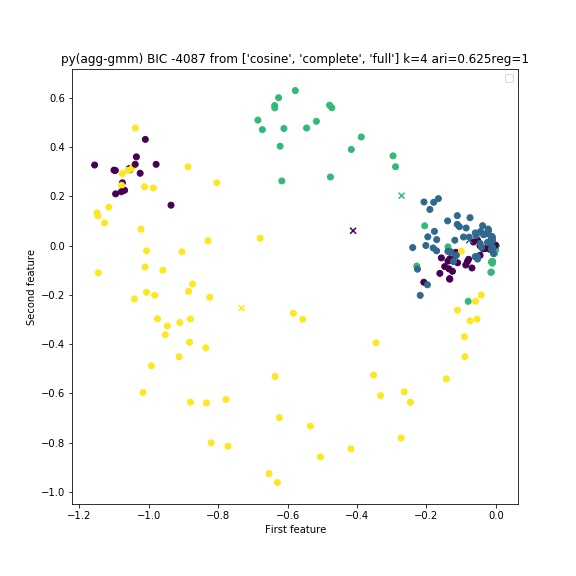
\includegraphics[width=\linewidth]{python_bic_k4.jpg}
\end{subfigure}
\begin{subfigure}[b]{0.3\linewidth}
  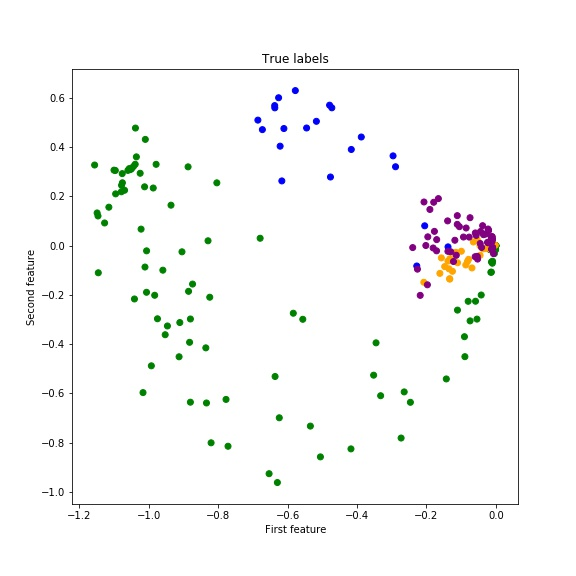
\includegraphics[width=\linewidth]{true.jpg}
\end{subfigure} 
\begin{subfigure}[b]{0.3\linewidth}
  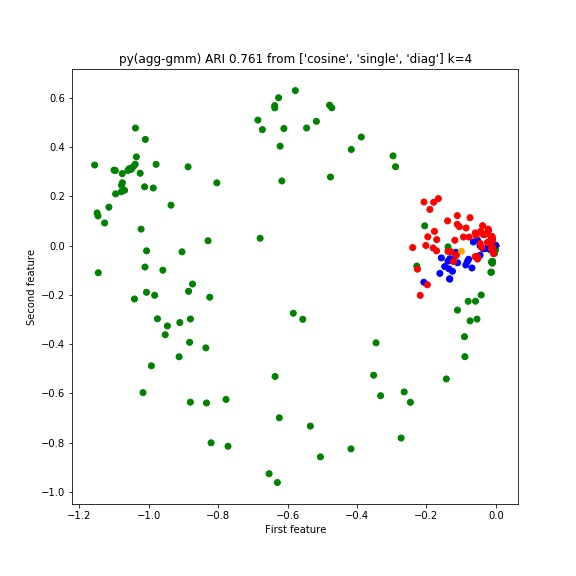
\includegraphics[width=\linewidth]{python_ari_k4.jpg}
\end{subfigure} 

\begin{subfigure}[b]{0.3\linewidth}
  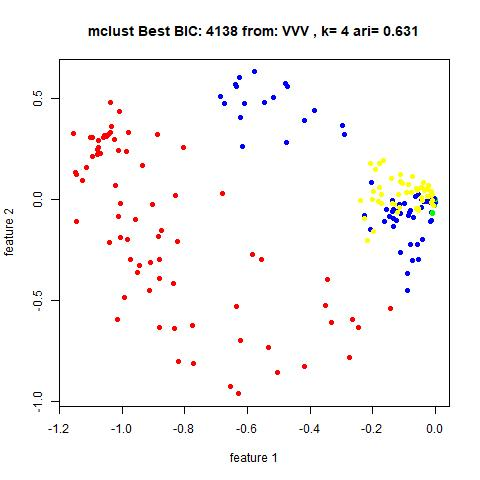
\includegraphics[width=\linewidth]{r_bic_k4.jpg}
\end{subfigure}
\begin{subfigure}[b]{0.3\linewidth}
  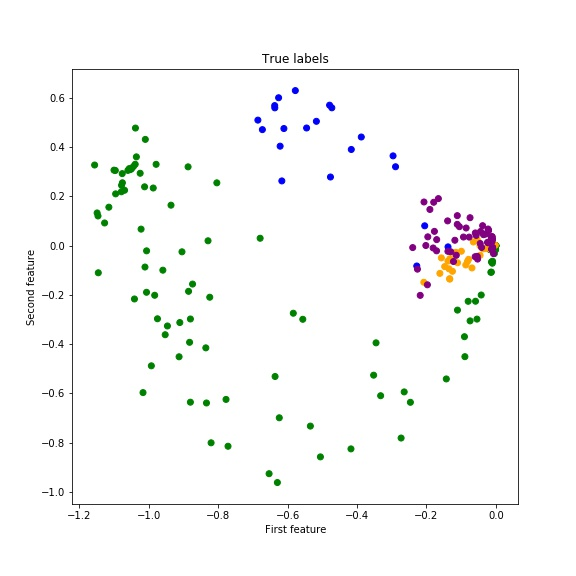
\includegraphics[width=\linewidth]{true.jpg}
\end{subfigure} 
\begin{subfigure}[b]{0.3\linewidth}
  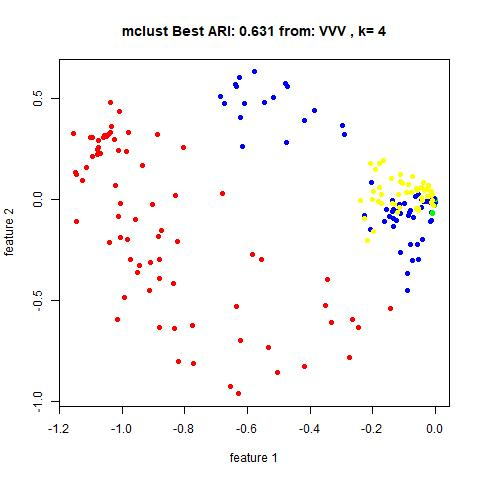
\includegraphics[width=\linewidth]{r_ari_k4.jpg}
\end{subfigure}
\end{figure}
Notes: \\
These plots are with k=4.\\
Top row is python, where I used HierarchicalAgglomeration assignments to initialize GMM EM. There are 40 possibilities total (manhattan/l1, euclidean/l2, cosine)metric x (ward, complete, average, single)linkage x (full,tied,diag,spherical)covariance, and ward linkage is only available with euclidean metric. Cosine affinity, which measures angles between points and single/complete linkage are not available in mclust.  \\ \\
Bottom row is mclust (14 total clustering possibilities), the VVV model is where each cluster has its own unconstrained variance. \\ \\
Remember that this is a single dataset, and I iterated through many clustering modes.

\newpage

\begin{figure}[h!]
\centering
\begin{subfigure}[b]{0.3\linewidth}
  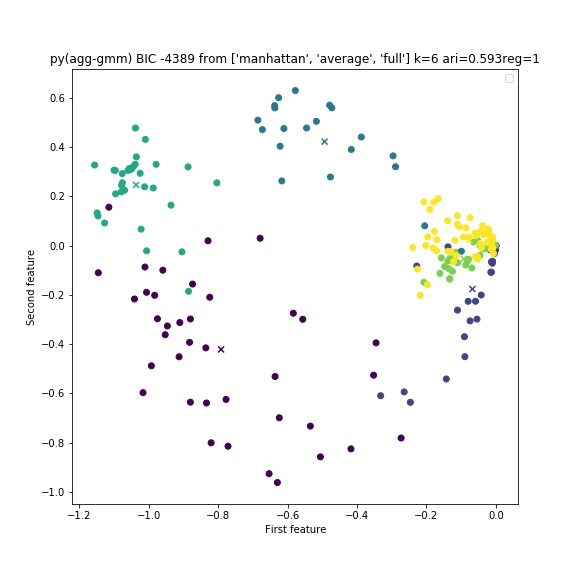
\includegraphics[width=\linewidth]{python_bic_k6.jpg}
\end{subfigure}
\begin{subfigure}[b]{0.3\linewidth}
  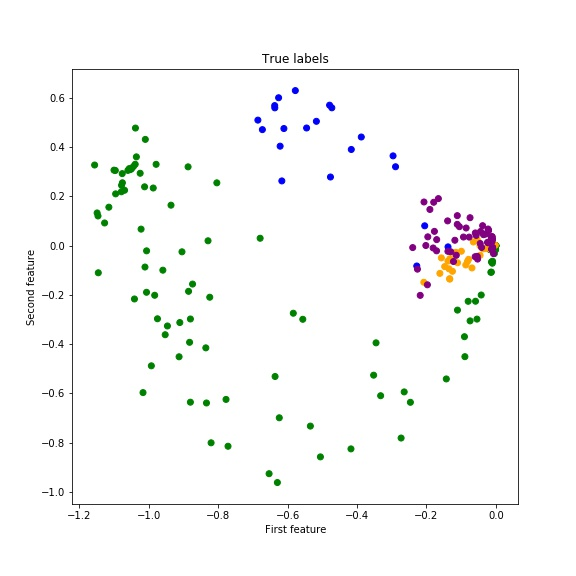
\includegraphics[width=\linewidth]{true.jpg}
\end{subfigure} 
\begin{subfigure}[b]{0.3\linewidth}
  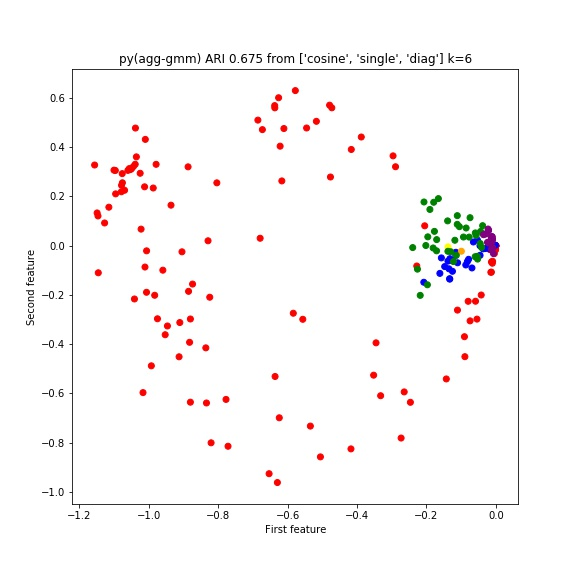
\includegraphics[width=\linewidth]{python_ari_k6.jpg}
\end{subfigure} 

\begin{subfigure}[b]{0.3\linewidth}
  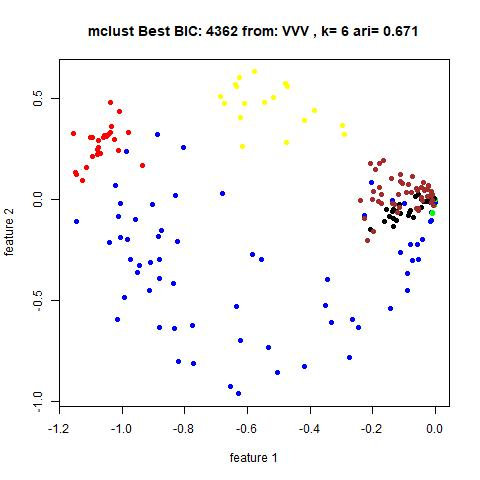
\includegraphics[width=\linewidth]{r_bic_k6.jpg}
\end{subfigure}
\begin{subfigure}[b]{0.3\linewidth}
  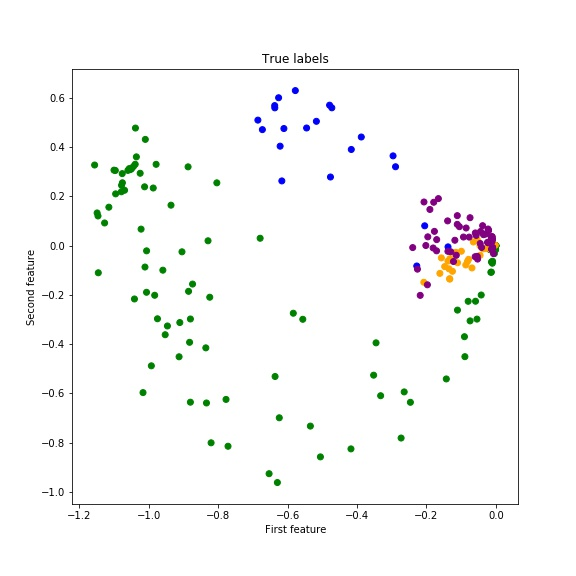
\includegraphics[width=\linewidth]{true.jpg}
\end{subfigure} 
\begin{subfigure}[b]{0.3\linewidth}
  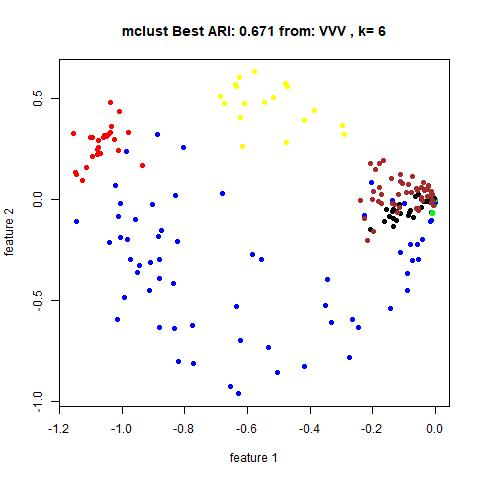
\includegraphics[width=\linewidth]{r_ari_k6.jpg}
\end{subfigure}
\end{figure}

k=6
\newpage

\begin{figure}[h!]
\centering
\begin{subfigure}[b]{0.4\linewidth}
  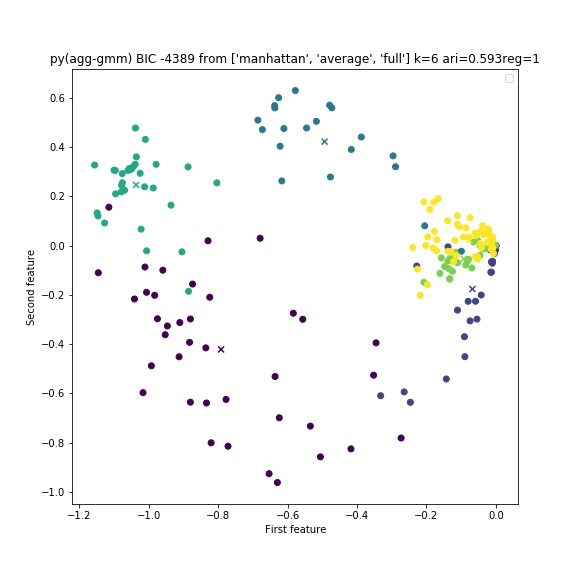
\includegraphics[width=\linewidth]{python_bic_allk.jpg}
\end{subfigure}
\begin{subfigure}[b]{0.4\linewidth}
  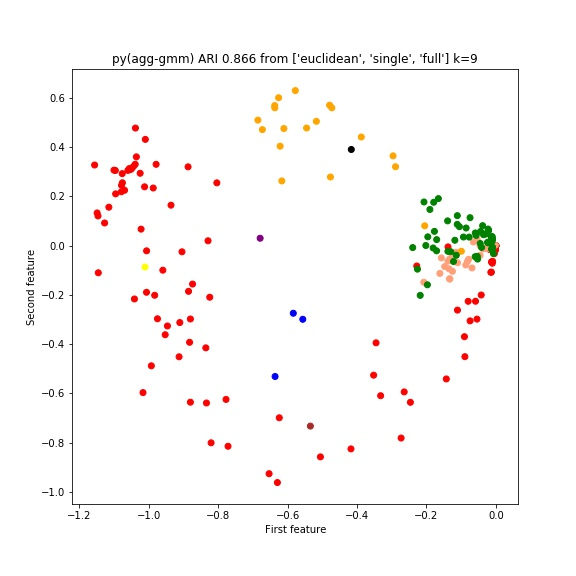
\includegraphics[width=\linewidth]{python_ari_allk.jpg}

\end{subfigure} 
\begin{subfigure}[b]{0.4\linewidth}
  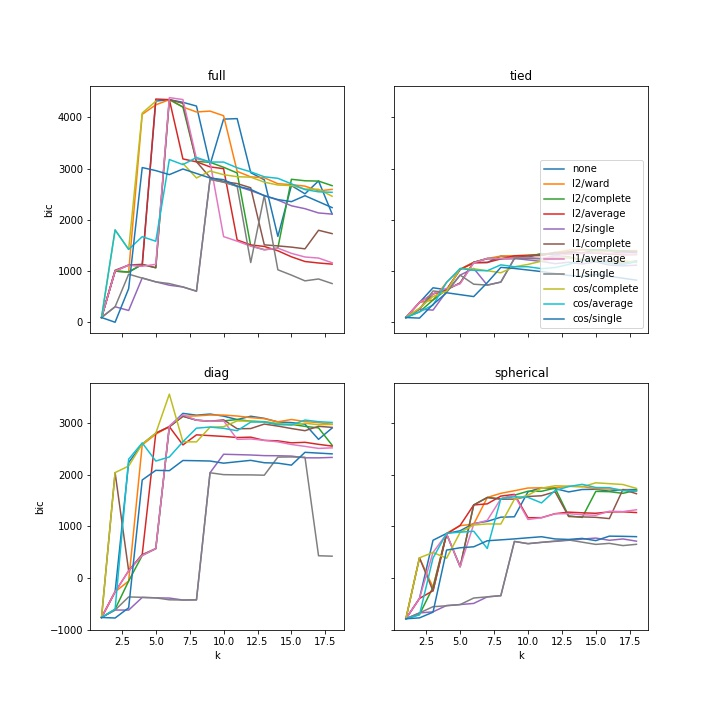
\includegraphics[width=\linewidth]{python_bicplot.jpg}
\caption{The subplots are divided by constraint used in GMM. The different lines are the agglomeration methods for initialization.}
\end{subfigure}
\end{figure} 

\newpage

\begin{figure}[h!]
\centering
\begin{subfigure}[b]{0.4\linewidth}
  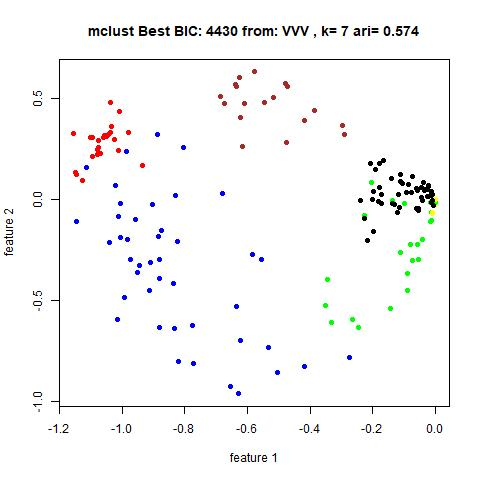
\includegraphics[width=\linewidth]{r_bic_allk.jpg}
\end{subfigure}
\begin{subfigure}[b]{0.4\linewidth}
  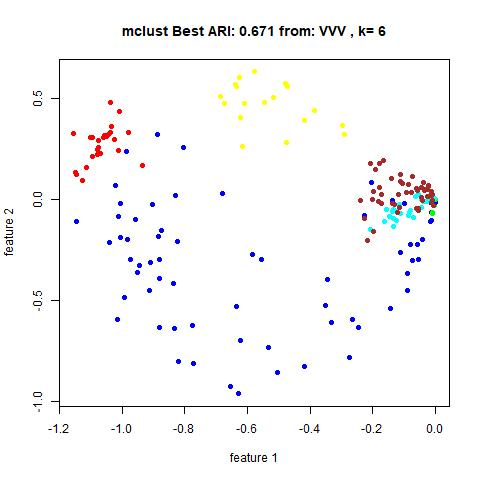
\includegraphics[width=\linewidth]{r_ari_allk.jpg}

\end{subfigure} 
\begin{subfigure}[b]{0.4\linewidth}
  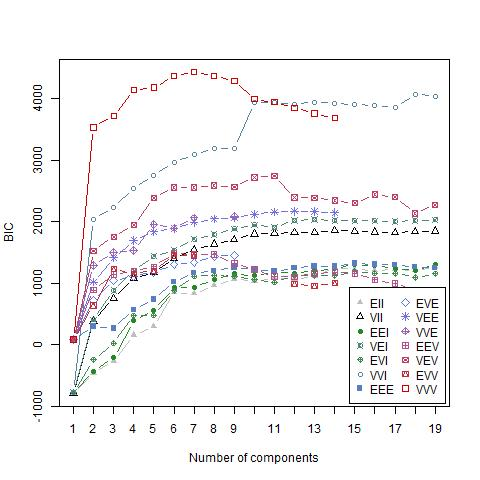
\includegraphics[width=\linewidth]{r_bicplot.jpg}
\end{subfigure}
\end{figure} 
\end{document}